\chapter{GPU-based Approximate $k$-Nearest Neighbor Computation} 
\label{chp:GLSH}

\section{Introduction}
Nearest neighbor search in high-dimensional spaces is an important problem in many areas, including databases, data mining and computer vision. It is a high-dimensional spatial proximity query used to perform similarity search between feature-rich data, such as digital audio, images or video, which are typically represented as high-dimensional feature vectors. The problem of exact or approximate $k$-nearest neighbor search is well studied in the literature. It is regarded as a challenging problem due to its intrinsic complexity and the accuracy issues that arise in terms of computing the appropriate $k$-nearest neighbors.

In terms of runtime cost, an ideal nearest neighbor query should take $\mathcal O(1)$ or $\mathcal O(\ln n)$ per-query time, because the size of the dataset (i.e., $n$) can be very large (e.g., $>$ 1 million). Moreover, the space required should be $\mathcal O(n)$ in order to handle large datasets. In terms of quality issues, each query should return $k$-nearest neighbor results that are close enough to the exact $k$-nearest neighbors computed via a brute-force, linear-scan approach that has a high $O(n)$ per-query complexity.

Most prior approaches for $k$-nearest neighbor computation can be slow on large high-dimensional datasets. For example, tree-based methods~\cite{Samet:2005:FMM} can compute accurate results efficiently on low dimensional datasets only. When the dimensionality exceeds $10$, these space partitioning-based methods can be slower than the brute-force approach~\cite{Weber:1998:QAP}. Methods based on Voronoi graphs are widely used in $k$-nearest query for spatial databases~\cite{Kolahdouzan:2004,Hu:2010:VSQ}, which have similar performance issues. Approximate nearest neighbor algorithms tend to compute neighbors that are close enough to the query item instead of the exact $k$-nearest neighbors, and have a lower runtime and space overhead than the exact algorithms~\cite{Kleinberg:1997}. For high-dimensional $k$-nearest neighbor search, one of the widely-used approximate methods is \emph{locality-sensitive hashing} (LSH)~\cite{Datar:2004:LHS}, which uses a family of hash functions to group or collect nearby items with a high probability into the same bucket. These buckets are stored in a hash table called LSH hash table. In order to perform a similarity query, LSH-based algorithms hash the query item into one bucket in the hash table and use the data items within that bucket as potential candidates for the final results. Moreover, the items in the bucket are ranked according to the exact distance to the query item in order to compute the $k$-nearest neighbors.
The final ranking computation among the candidates is called the \emph{short-list search}, which is regarded as the main bottleneck in LSH-based algorithms. However, there is relatively little work on accelerating the performance of short-list search or the overall performance of the LSH-based $k$-nearest neighbor algorithms.

\subsection{Main Results}
In this chapter, we present a GPU-based parallel algorithm for efficient $k$-nearest neighbor search in a high-dimensional space. We use the Bi-level LSH framework~\cite{BilevelLSH2011}, which offers improved quality compared to prior LSH methods and exploits the high number of cores and data parallelism within GPUs to improve the performance of LSH hash table construction and short-list search. For LSH hash table construction, we compute the LSH hashing value for each data item in parallel and then store these values using a cuckoo hashing table. In the query step, we use a work queue based algorithm to significantly accelerate short-list search, for single-query as well as multi-query cases. In particular, our GPU-based parallel Bi-level LSH algorithm can provide more than 40X acceleration over single-core CPU implementations that do not perform SIMD optimizations.

\subsection{Organization}
The rest of this chapter is organized as follows. We give an overview of LSH computation and briefly survey prior methods related to KNN computation in Section~\ref{sec:6:related}. Section~\ref{sec:6:overview}
gives an overview of Bi-level LSH scheme. In Section~\ref{sec:6:primitive}, we describe some parallel primitives that are used in our GPU-based algorithm. We present our detailed GPU-based Bi-level LSH algorithm in Section~\ref{sec:6:parallel}, and highlight its performance in Section~\ref{sec:6:res}.

\section{Background and Related Work}
\label{sec:6:related}

In this section, we first give an overview of LSH based $k$-nearest neighbor computation. Next, we give a brief survey of different algorithms used for KNN query.

\subsection{Basic LSH}
\label{sec:6:related:basic}
Given a metric space $(\mathbb X, \|\cdot\|)$ and a database $S \subseteq \mathbb X$, for any given query $\mathbf v \in \mathbb X$, the $k$-nearest neighbor algorithm computes a set of $k$ points $I(\mathbf v) \subseteq S$ that are closest to $\mathbf v$. We assume that $\mathbb X$ is embedded in a $D$-dimensional Euclidean space $\mathbb{R}^D$ and each item is represented as a high-dimensional vector, i.e., $\mathbf v = (v_1, ..., v_D)$.

The basic LSH algorithm is an approximate method to compute $k$-nearest neighbors, which uses $M$ ($M \ll D$) hash functions $h_1(\cdot), ..., h_M(\cdot)$ to transform $\mathbb{R}^D$ into a lattice space $\mathbb{Z}^M$ and distributes each data item into one lattice cell:
\begin{equation}
H(\mathbf v) = \langle h_1(\mathbf v), h_2(\mathbf v), ..., h_M(\mathbf v) \rangle.
\end{equation}
The lattice space is usually implemented as a hash table, since many of the cells may be empty. LSH algorithms have been developed for several distance measures, such as $l_p$ distance. For $l_p$ space, $p \in (0, 2]$~\cite{Datar:2004:LHS},
\begin{equation}
\label{eq:6:hash:basic}
h_i(\mathbf v) = \lfloor \frac{\mathbf a_i \cdot \mathbf v + b_i}{W} \rfloor,
\end{equation}
where the $D$-dimensional vector $\mathbf a_i$ consists of i.i.d. entries from Gaussian distribution $N(0, 1)$ and $b_i$ is drawn from a uniform distribution $U[0, W)$. $M$ and $W$ control the dimension and size of each lattice cell and therefore control the locality sensitivity of the hash functions.
In order to achieve high quality results in terms of accuracy, $L$ hash tables are used with independent dim-$M$ hash functions $H(\cdot)$. Given a query item $\mathbf v$, we first compute its hash code using $H(\mathbf v)$ and locate the hash bucket that contains $\mathbf v$. All the points in the bucket will belong to its potential $k$-nearest neighbor candidate set and we represent that set as $A(\mathbf v)$. Next, we perform a local scan on $A(\mathbf v)$ to compute the $k$-nearest neighbors $I(\mathbf v)$. This step is called short-list search and is the main bottleneck of the LSH framework.

There are several known metrics used to measure the performance of a $k$-nearest neighbor search algorithm. First is the \emph{recall ratio}, i.e., the percentage of the exact $k$-nearest neighbors $N(\mathbf v)$ in the returned results $I(\mathbf v)$:
\begin{equation}
\label{eq:6:recall}
\rho(\mathbf v) = \frac{|N(\mathbf v) \cap I(\mathbf v)|}{|N(\mathbf v)|} = \frac{|N(\mathbf v) \cap A(\mathbf v)|}{|N(\mathbf v)|},
\end{equation}
where $N(\mathbf v)$ can be computed using any exact $k$-nearest neighbor approach and serves as the ground-truth.

The second metric is the \emph{error ratio}~\cite{Gionis:vldb:99}, i.e., the relationship between $\mathbf v$'s distance to $N(\mathbf v)$ and $I(\mathbf v)$:
\begin{equation}
\label{eq:6:error}
\kappa(\mathbf v) = \frac{1}{k} \sum_{i=1}^k \frac{\|\mathbf v -N(\mathbf v)_i\|}{\| \mathbf v - I(\mathbf v)_i\|},
\end{equation}
where $N(\mathbf v)_i$ or $I(\mathbf v)_i$ is $\mathbf v$'s $i$-th nearest neighbor in $N(\mathbf v)$ or $I(\mathbf v)$. We use recall and error ratios to measure the quality of the LSH algorithm; our goal is to compute the $k$-nearest neighbors with large recall and error ratios, which are both within $[0, 1]$ interval.

The final metric is the \emph{selectivity}~\cite{Dong:2008:MLP}, which measures the runtime cost of the short-list search:
\begin{equation}
\label{eq:6:selectivity}
\tau(\mathbf v) = |A(\mathbf v)| / |S|,
\end{equation}
where $|S|$ is the size of the dataset.

\subsection{Variations of LSH}
Many techniques have been proposed to improve the basic LSH algorithm. LSH-forest~\cite{Bawa:2005:LFS} avoids tuning of the parameter $M$ by representing the hash table as a prefix tree and the parameter $M$ is computed based on the depth of the corresponding prefix-tree leaf node. Multi-probe LSH~\cite{Lv:2007:MLE} systematically probes the buckets near the query points in a query-dependent manner, instead of only probing the bucket that contains the query point. It can obtain a higher recall ratio with fewer hash tables, but may result in larger selectivity from additional probes. \cite{Dong:2008:MLP} construct a statistical quality and runtime model with a small sample dataset, and then compute $M$ and $W$ that can result in a good balance between high recall and low selectivity. \cite{Joly:2008:PML} improve the multi-probe LSH by using prior information collected from a sampled dataset.

Many approaches have been proposed to design better hash functions. $\mathbb Z^M$ lattice may suffer from the curse of dimensionality: in a high dimensional space, the \emph{density} of $\mathbb Z^M$ lattice, i.e., the ratio between the volume of one $\mathbb Z^M$ cell and the volume of its inscribed sphere, increases very quickly when the dimensionality increases. In order to overcome these problems, lattices with densities close to one are used as space quantizers, e.g., $E_8$-lattice~\cite{Jegou:2008} and Leech lattice~\cite{Andoni:2006:NHA} are used for dim-8 and dim-24 data items, respectively.




\section{Bi-level Locality-Sensitive Hashing}
\label{sec:6:overview}

In this section, we first give an overview of our new Bi-level LSH scheme. Next we address some issues in designing efficient GPU-based parallel Bi-level LSH algorithm.

\subsection{Bi-level LSH Scheme}
\label{sec:6:overview:lsh}
The Bi-level LSH scheme~\cite{BilevelLSH2011} is designed to obtain better performance and accuracy on datasets composed of multiple clusters with different data distributions. The approach takes into account the properties of datasets and can generate high quality LSH codes. It can also reduce the performance/quality variance caused by randomness in the LSH scheme or different queries.

An overview of our algorithm is shown in Figure~\ref{fig:6:overview} and includes two levels.
In the first level, we construct a \emph{random projection tree} (RP-tree)~\cite{yoav:nips:2007,Dasgupta:2008}, which is a space-partitioning data structure that is used to organize high-dimensional data items into several subsets. In a RP-tree, each subset is represented as one leaf node. Compared to other methods such as Kd-tree or K-means, RP-tree has many good properties, including fast convergence speed, guaranteed `roundness' of leaf nodes~\cite{Dasgupta:2008,aman:nips:2010}, etc. These properties are useful for generating compact LSH code and reducing the algorithm's performance/quality variance.
\begin{figure}[t]
  \centering
  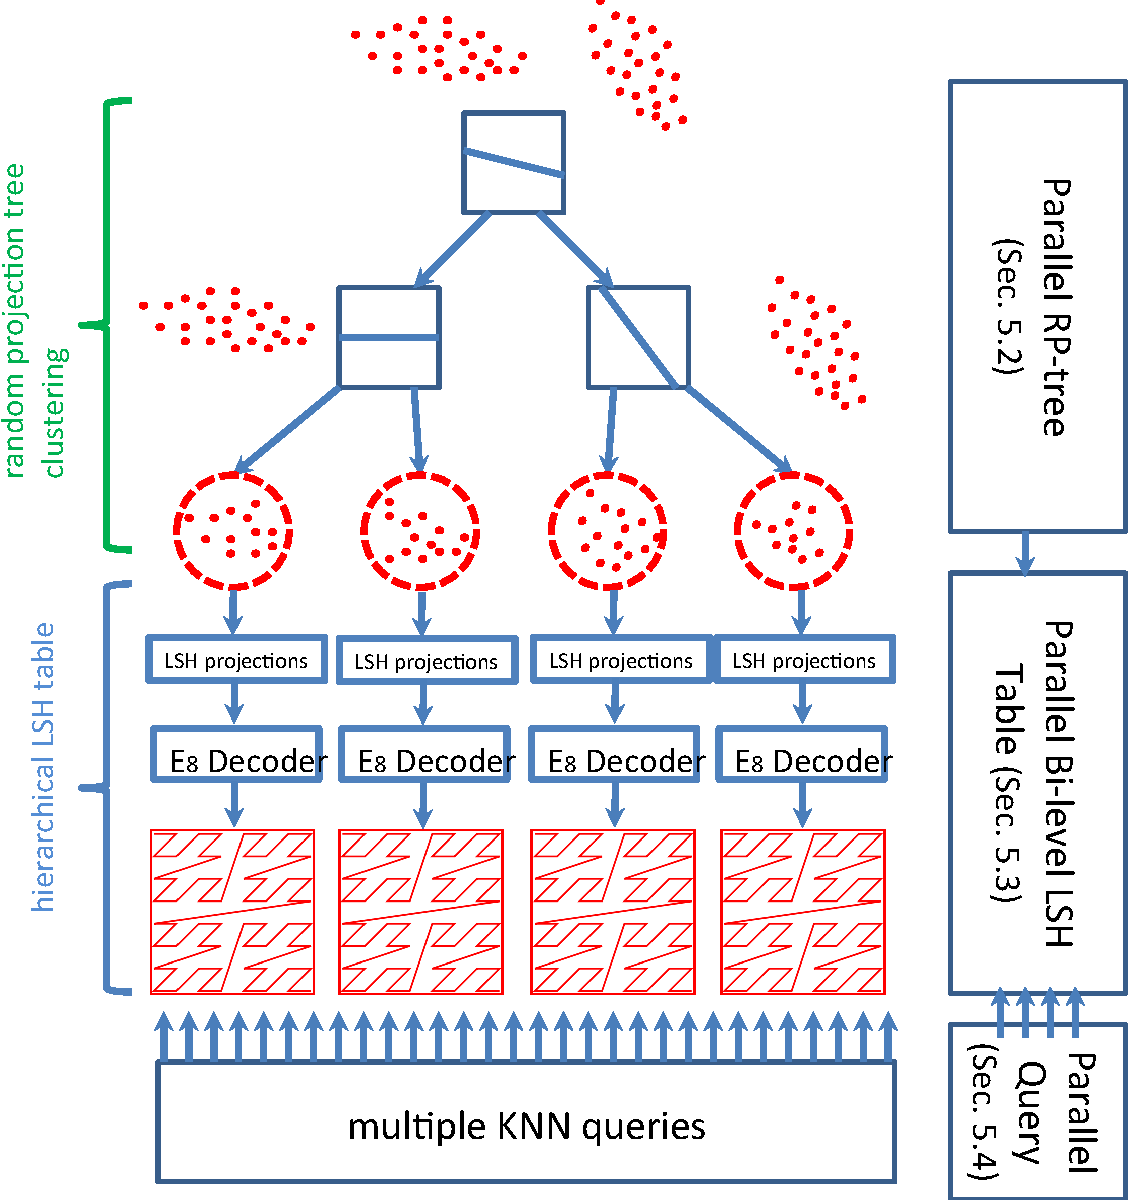
\includegraphics[width=0.8\linewidth]{figs/6/overview.pdf}
  \caption[Bi-level LSH framework]{\label{fig:6:overview} The framework for Bi-level LSH. The first level is the random projection tree. The second level is the hierarchical lattice for each RP-Tree leaf node. Both levels are parallelized utilizing the multiple cores on a GPU. }
\end{figure}
During the second level, we construct locality-sensitive hash (LSH) tables for each of the subsets generated in the first level. Unlike prior methods, our LSH table has a hierarchical structure that is constructed using a Morton curve. The hierarchical LSH table can reduce the performance/quality variance among different queries: for query within regions with high data density, the algorithm only needs to search the buckets nearby; for query within regions with low data density, the algorithm can automatically search in far away buckets to provide enough $k$-nearest neighbor candidates. We also enhance the hierarchy using an $E_8$ lattice , which can overcome $\mathbb Z^M$ lattice's drawbacks for high-dimensional datasets and can improve the accuracy of the results.

For each item $\mathbf v$ in the dataset, our method finds the RP-tree leaf node $\text{RP-tree}(\mathbf v)$ that contains $\mathbf v$ and computes its LSH code $H(\mathbf v)$ using LSH parameters for that subset in the second level. As a result, our Bi-level LSH scheme decomposes the basic LSH code into two parts: the RP-tree leaf node index and the LSH code corresponding to the subset, i.e., $\tilde{H}(\mathbf v) = (\text{RP-tree}(\mathbf v), H(\mathbf v))$. Such a Bi-level code can remove the redundancy in the traditional LSH code~\cite{BilevelLSH2011}.
The resulting Bi-level LSH code $\tilde{H}(\mathbf v)$ is stored in a hash table.

Given one query, we first traverse the RP-tree to find the leaf node that it belongs to, and then compute its Bi-level LSH code within the subset. Based on the hash code, we compute the buckets in the hash table with same or similar hash codes, which are used as the candidates for $k$-nearest neighbors. Finally, we perform short-list search on the candidates to compute the $k$ items closest to the query. For more details of the Bi-level LSH algorithm, such as how $E_8$ lattice and Morton curve hierarchy are integrated into the LSH framework, please refer to~\cite{BilevelLSH2011}.

\subsection{GPU and Parallel LSH}
Many techniques used in previous LSH algorithms are not suitable for current GPU architecture. For example, the prefix tree used in LSH-forest~\cite{Bawa:2005:LFS} and the PCA used in spectral hashing~\cite{weiss:nips:2008} are not the best candidates for GPU parallelization. When using LSH schemes to compute $k$-nearest neighbors for multiple queries, the simplest way to parallelize is by using independent GPU threads for different KNN queries.
However, such per-thread per-query approach has several drawbacks. First, the multi-probe technique~\cite{Lv:2007:MLE} uses a query-dependent sequence to decide the optimal visiting order for nearby hash buckets. This will cause branch divergence among threads and will reduce the overall performance. Second, different queries may result in intermediate data structures of varying sizes (i.e., short-list with different sizes), which results in work-load imbalance among GPU cores: some cores are busy performing exact distance comparisons among candidates while others may be idle. Finally, this scheme may leave many GPU processors idle when the number of queries is small.

\section{GPU Primitives}
\label{sec:6:primitive}
In this section, we present the underlying parallel primitives that are used frequently by our GPU-based KNN algorithm.

\subsection{Standard Primitives}
The following primitives have been used in the literature and can be efficiently implemented on current GPUs.

\noindent {\bf{Gather and Scatter}} \ \ As defined in~\cite{He:2007:EGS}, scatter rearranges the elements in an array $R_{in}$ to another array $R_{out}$ according to a location array $index$ and gather does the opposite of scatter. Usually the location array is a permutation array.

\noindent \fbox{\begin{minipage}[t]{0.9\linewidth} {\bf{Primitive:}} $R_{out}$ = \texttt{scatter}($R_{in}$, $index$) \\ {\bf{Input:}} $R_{in}$[$1$:$n$], $index$[$1$:$n$] \\	{\bf{Output:}} $R_{out}$[$1$:$n$] \\ {\bf{Function:}} $R_{out}[index[i]] = R_{in}[i]$, $i = 1, ..., n$ \end{minipage}}

\noindent \fbox{\begin{minipage}[t]{0.9\linewidth} {\bf{Primitive:}} $R_{out}$ = \texttt{gather}($R_{in}$, $index$) \\ {\bf{Input:}} $R_{in}$[$1$:$n$], $index$[$1$:$n$] \\	{\bf{Output:}} $R_{out}$[$1$:$n$] \\ {\bf{Function:}} $R_{out}[i] = R_{in}[index[i]]$, $i = 1, ..., n$ \end{minipage}}

\noindent {\bf{Compact/Pack}} \ \ Compact or pack scatters the elements which are marked as true~\cite{Horn:2005:gpugems}.

\noindent \fbox{\begin{minipage}[t]{0.9\linewidth} {\bf{Primitive:}} $R_{out}$ = \texttt{compact}($R_{in}$, $F$, $index$) \\ {\bf{Input:}} $R_{in}$[$1$:$n$], $F$[$1$:$n$], $index$[$1$:$n$] \\ {\bf{Output:}} $R_{out}$[$1$:$m$] \\ {\bf{Function:}} if $F[i] = 1$, $R_{out}[index[i]] = R_{in}[i]$, $i = 1, ..., n$ \end{minipage}}

\noindent {\bf{Reduction and Segmented-Reduction}} \ \ Reduction takes a sequence of values and applies a binary operator on the array to distill a single value. The associative operator includes $+$, $\max$, $\min$, etc. Segmented-reduction performs reduction operation on elements with the same segmentation index~\cite{Zhou:2008:RKC}.

\noindent \fbox{\begin{minipage}[t]{0.9\linewidth} {\bf{Primitive:}} $R_{out}$ = \texttt{reduction}($R_{in}$, $\bigoplus$)\\ {\bf{Input:}} $R_{in}$[$1$:$n$], associative operator $\bigoplus$ \\ {\bf{Output:}} $R_{out}$ \\ {\bf{Function:}} $R_{out} = \bigoplus_{i=1}^n R_{in}[i]$ \end{minipage}}

\noindent \fbox{\begin{minipage}[t]{0.9\linewidth} {\bf{Primitive:}} $R_{out}$ = \texttt{segmented-reduction}($R_{in}$, $segId$, $\bigoplus$)\\ {\bf{Input:}} $R_{in}$[$1$:$n$], $segId$[$1$:$n$], associative operator $\bigoplus$ \\ {\bf{Output:}} $R_{out}$[$1$:$m$] \\ {\bf{Function:}} $R_{out}[i] = \bigoplus_{segId[j] = i} R_{in}[j]$, $i = 1,..., m$ \end{minipage}}

\noindent {\bf{Scan and Segmented-Scan}} \ \ Scan~\cite{Horn:2005:gpugems}, also called prefix-sums, takes a binary operator, an identity function and an array and returns a new array in which each element is the sum of all previous elements (sum is defined relative to the associative operator). The associative operator includes $+$, $\max$, $\min$, etc. There are two types of scan, exclusive or inclusive scan. Inclusive scan includes the element at the current position while exclusive scan does not.

\noindent \fbox{\begin{minipage}[t]{0.9\linewidth} {\bf{Primitive:}} $R_{out}$ = \texttt{scan}($R_{in}$, $\bigoplus$) \\ {\bf{Input:}} $R_{in}$[$1$:$n$], associative operator $\bigoplus$ \\ {\bf{Output}:} $R_{out}$[$1$:$n$] \\ {\bf{Function:}} $R_{out}[i] = \bigoplus_{j < i} R_{in}[j]$ (exclusive) or $R_{out}[i] = \bigoplus_{j \leq i} R_{in}[j]$ (inclusive), $i = 1, ..., n$ \end{minipage}}

\noindent \fbox{\begin{minipage}[t]{0.9\linewidth} {\bf{Primitive:}} $R_{out}$ = \texttt{segmented-scan}($R_{in}$, $segId$, $\bigoplus$) \\ {\bf{Input:}} $R_{in}$[$1$:$n$], $segId$[$1$:$n$], associative operator $\bigoplus$ \\ {\bf{Output:}} $R_{out}$[$1$:$n$] \\ {\bf{Function:}} $R_{out}[i] = \bigoplus_{j < i, segId[j] = segId[i]} R_{in}[j]$ (exclusive) or $R_{out}[i] = \bigoplus_{j \leq i, segId[j] = segId[i]} R_{in}[j]$ (inclusive), $i = 1, ..., n$ \end{minipage}}

\noindent {\bf{Radix sort}} \ \ Radix sort~\cite{Sengupta:2007:SPG} rearranges an array in ascending order in linear time. It can also sort an associative array according to the keys where the associative value is often the element's position before and after sorting.

\noindent \fbox{\begin{minipage}[t]{0.9\linewidth} {\bf{Primitive:}} \texttt{radix-sort}($keys$, $values$[optional]) \\ {\bf{Input:}} $keys$[$1$:$n$] and $values$[$1$:$n$] \\ {\bf{Output:}} Sorted $keys$[$1$:$n$] and updated $values$[$1$:$n$] \\ {\bf{Function:}} radix sort, $keys$ stores the comparison key value for each element, while $values$ stores the associative values \end{minipage}}

\subsection{Primitives for Clustered Data}
In addition to the aforementioned primitives, we have developed new GPU primitives for our Bi-level LSH algorithm. According to Section~\ref{sec:6:overview:lsh}, we frequently perform operations
on the entire dataset which has already been partitioned into several groups by the RP-tree. These operations include: (1) sort the whole
dataset, but keep the relative order between different groups; (2) compute the sum, mean or median for each group. We can perform such operations for each group sequentially, but that may not achieve the peak performance on parallel architectures like GPUs, especially when the number of groups is large. Moreover, the data items belonging to the same group are clustered together to locate in adjacent positions on the memory and we know the beginning position $B$ and number of items $N$ of each group. Based on this information, we can design more efficient algorithms on the partitioned data instead of simply applying the segmented version of standard primitives (e.g., segmented-scan or segmented-reduct). In order to distinguish from segmented primitives, we name the operations on clustered data sets as \emph{clustered primitives}.

\noindent {\bf{Clustered-sort}} \ \ Clustered-sort rearranges a partitioned array in ascending order in parallel but keeps the relative order between the different groups.

\noindent \fbox{\begin{minipage}[t]{0.9\linewidth} {\bf{Primitive:}} \texttt{clustered-sort}($keys$,$groupId$,$values$[optional])\\ {\bf{Input:}} $keys$[$1$:$n$], $groupId$[$1$:$n$], $values$[$1$:$n$] \\ {\bf{Output:}} $keys$[$1$:$n$] and $values$[$1$:$n$] \\ {\bf{Function:}} Radix sort but also keep the relative order between groups \end{minipage}}

One way to implement clustered-sort is via standard radix sorting on data ($groupId \times keys$) according to dictionary order, i.e., \texttt{radix-sort}($groupId \times keys$, $values$). Another method is to modulate the $keys$ using $groupId$ values so that elements belonging to different groups can be distinguished according to different $keys$ values. For example, we can change $keys[i]$ to be $keys'[i] = keys[i] + groupId[i] \cdot \Delta$, where $\Delta$ = \texttt{reduct}($keys$, $\max$). Then we only perform standard radix sort on the modulated keys, i.e., \texttt{radix-sort}($keys'$, $values$). Both methods can be implemented efficiently on GPUs, but the second one is more memory efficient.

\noindent {\bf{Clustered-sum}} \ \ Clustered-sum computes the sum of elements in each of the $m$ groups. We first perform scan primitive on the entire dataset and then perform compact primitive on the scan results to obtain the summation for each group.

\noindent \fbox{\begin{minipage}[t]{0.9\linewidth} {\bf{Primitive:}} $R_{out}$ = \texttt{clustered-sum}($R_{in}$, $B$, $N$) \\ {\bf{Input:}} $R_{in}$[$1$:$n$], group start positions $B$[$1$:$m$] and group sizes $N$[$1$:$m$]  \\ {\bf{Output:}} per-group summation $R_{out}$[$1$:$m$] \\ {\bf{Function:}} \\ $R_{temp}$ = \texttt{inclusive-scan}($R_{in}$, $\max$) \\ $index[i] = B[i] + N[i]$, $i = 1,...,m - 1$; $index[m]$ = \texttt{reduction}($N$, $+$) \\ $R_{out}$ = \texttt{compact}($R_{temp}$, $index$) \end{minipage}}

The GPU primitives used to compute mean or median of the clustered data items are similar to clustered-sum.


\section{Parallel Bi-level Locality Sensitive Hashing}
\label{sec:6:parallel}
In this section, we describe the parallel Bi-level LSH algorithm.

\subsection{First Level: RP-tree}
During the first level, we use \emph{random projection tree} (RP-tree)~\cite{yoav:nips:2007,Dasgupta:2008} to divide the dataset into several small clusters with good properties for subsequent LSH-based operations. The RP-tree construction algorithm is similar to Kd-tree computation: given a data set, we use a split rule to divide it into two subsets, which are split recursively until the resulting tree has a desired depth. Kd-tree chooses a coordinate direction (typically the coordinate with the largest spread) and then splits the data according to the median value for that coordinate. Unlike Kd-tree, RP-tree projects the data onto a randomly chosen unit direction and then splits the set into two roughly equal-sized sets using new split rules. \cite{Dasgupta:2008} have proposed two rules for RP-trees: RP-tree max and RP-tree mean. The difference between the two rules is that RP-tree mean occasionally performs a different kind of split based on the distance from the mean of the coordinates. In practice, we observe that RP-tree mean rule tends to compute the $k$-nearest neighbor results with better quality in terms of the recall ratio. Therefore, we use RP-tree mean rule to construct the RP-tree for Bi-level LSH.

To apply RP-tree mean rule, we need to efficiently compute $\Delta(S)$, the diameter for a given point set $S$ in a high-dimensional space, which is in fact as difficult as the original $k$-nearest neighbor query. There are many known algorithms for approximating the diameter efficiently, and we use the iterative method proposed by~\cite{Egecioglu:1989:ADS}. In practice, it converges fast to an approximation with good precision and can be easily parallelized. The diameter computation algorithm uses a series of $m$ values $r_1, ..., r_m$ to approximate the diameter for a point set $S$, where $m \leq |S|$. It can be proved that $r_1 < r_2 < ... < r_m \leq \Delta(S) \leq \min(\sqrt{3}r_1, \sqrt{5-2\sqrt{3}}r_m)$~\cite{Egecioglu:1989:ADS}. In practice, we find that $r_m$ is usually a good approximation of $\Delta(S)$ even when $m$ is small (e.g., 40). The time complexity of this approximate diameter algorithm is $O(m|S|)$ and we can construct each level of the RP-tree in time that is linear in the size of the entire dataset. As a result, the overall complexity to partition the dataset into $g$ groups is $O(\log(g) n)$. The parallel algorithm for approximate diameter computation is highlighted in Algorithm~\ref{algo:6:diameter-parallel}.

During the construction of RP-tree, we start from all elements in one group and then compute the mean and diameter of each group to decide the split vector and split position. Then we compute the new group index of each element according to whether it lies on the right or left side of the split line. Finally we perform clustered-sort on the data to partition the dataset into two. We repeat this process until the algorithm reaches the appropriate depth of a RP-tree. The parallel tree construction algorithm is shown in Algorithm~\ref{algo:6:rptree-parallel}.

\begin{algorithm}[htb]
    \caption{Parallel Approximate Diameter Computation}
    \label{algo:6:diameter-parallel}
    \begin{algorithmic}[1]
    \STATE Input: Dim-$D$ data set $S$[$1$:$n$] partitioned into $m$ groups; group indices $G$[$1$:$n$], group begin positions $B$[$1$:$m$]; group sizes $N$[$1$:$m$]
    \STATE randomly select one point per group to make the query set $P$[$1$:$m$] {\bf{in parallel}}
    \STATE initialize the active mark set $I$[$1$:$m$] to all $1$ (all active)
    \STATE initialize the distances to query point $dist$[$1$:$n$] to $0$
    \STATE initialize element positions $index$[$1$:$n$] to $[1,2,...,n]$
    \STATE compute the group end positions $E$[$1$:$m$] from $B$ and $N$ {\bf{in parallel}}
    \LOOP
        \STATE compute the distance of each element to the query point with the same group index {\bf{in parallel}}: $dist[i] \leftarrow \|P[G[i]] - S[index[i]]\|$, $i = 1,...,n$
        \STATE \texttt{clustered-sort}($dist$, $G$, $index$)
        \STATE $index_c$ = \texttt{compact}($index$, $E$)
        \STATE set $Q$ and $\Psi$ store the compact results {\bf{in parallel}}: $Q[i] = S[index_c[i]]$ and $\Psi[i] = dist[index_c[i]]$
        \STATE compute the distance to the query point in $Q$ {\bf{in parallel}}: $dist[i] \leftarrow \|Q[G[t_i]] - S[index[i]]\|$
        \STATE \texttt{clustered-sort}($dist$, $G$, $index$)
        \STATE $index_c$ = \texttt{compact}($index$, $E$)
        \STATE set $Q'$ and $\Psi'$ store the compact results {\bf{in parallel}}: $Q'[i] = S[index_c[i]]$ and $\Psi'[i] = dist[index_c[i]]$
        \STATE remove points in $P$ and $Q$ by setting $0$ in corresponding position in $I$
        \STATE update $P$ {\bf{in parallel}}: $P[i] \leftarrow Q[i] + \frac{\Psi[i]}{\Psi'[i]} (P[i] - Q[i])$
        \STATE $n \leftarrow$ \texttt{reduction}($I$, $+$)
        \STATE \textbf{break} \textbf{if} $n = 0$ or all elements in $\Psi'$ starts decreasing.
    \ENDLOOP
    \STATE \textbf{return} $\Psi'$
    \end{algorithmic}
\end{algorithm}

\begin{algorithm}[htb]
    \caption{Parallel RP-tree Construction}
    \label{algo:6:rptree-parallel}
    \begin{algorithmic}[1]
    \STATE Input: Dim-$D$ data set $S$[$1$:$n$]; element positions $index$[$1$:$n$], group indices $G$[$1$:$n$]; RP-tree depth $depth$
    \STATE Initialize $G$ to all 1
    \STATE Initialize $index$ to $[1,2,...,n]$
    \FOR{$i = 1$ to $depth$}
        \STATE compute properties (mean, diameter, average diameter) needed for each group {\bf{in parallel}}
        \STATE decide the split vector and position for each group, according to RP-tree mean rule, which need parallel median and mean operations
        \STATE update the group index for each item according to split vector/position {\bf{in parallel}}: if go to left node, $G[i] \leftarrow 2 G[i] - 1$, otherwise $G[i] \leftarrow 2 G[i]$
        \STATE \texttt{clustered-sort}($S$, $G$, $index$)
    \ENDFOR
    \STATE \textbf{return} $S$, $index$ and $G$
    \end{algorithmic}
\end{algorithm}

\subsection{LSH Hash Table}
In the second level of the bi-level algorithm, we construct LSH hash table for each leaf node cell calculated during the first level.
The LSH code of one item and its leaf node index composes its Bi-level LSH code, i.e., $\tilde{H}(\mathbf v) = (\text{RP-tree}(\mathbf v), H(\mathbf v))$.

The LSH table is implemented as a linear array along with an indexing table. The linear array contains the Bi-level LSH codes of all the items in the dataset, which have been sorted to collect items with same LSH codes together. All the data items with the same LSH code constitute a bucket which is described by the start and end positions of the bucket (i.e., the bucket interval) in the sorted linear array. As each bucket uniquely corresponds to one LSH code, we can use the terminology `bucket' and `unique LSH code' in the same sense. The indexing table corresponds to a cuckoo hash table with each key as one LSH code and the value associated with the key is the corresponding bucket interval for the LSH code in the linear array. In practice, the key, a dim-$M$ LSH code, is compressed to a dim-1 key by using another hash function. The structure of the LSH hash table is shown in Figure~\ref{fig:6:hashtable}, which is implemented as a cuckoo hashing table on GPUs.

\begin{figure}[htb]
  \centering
  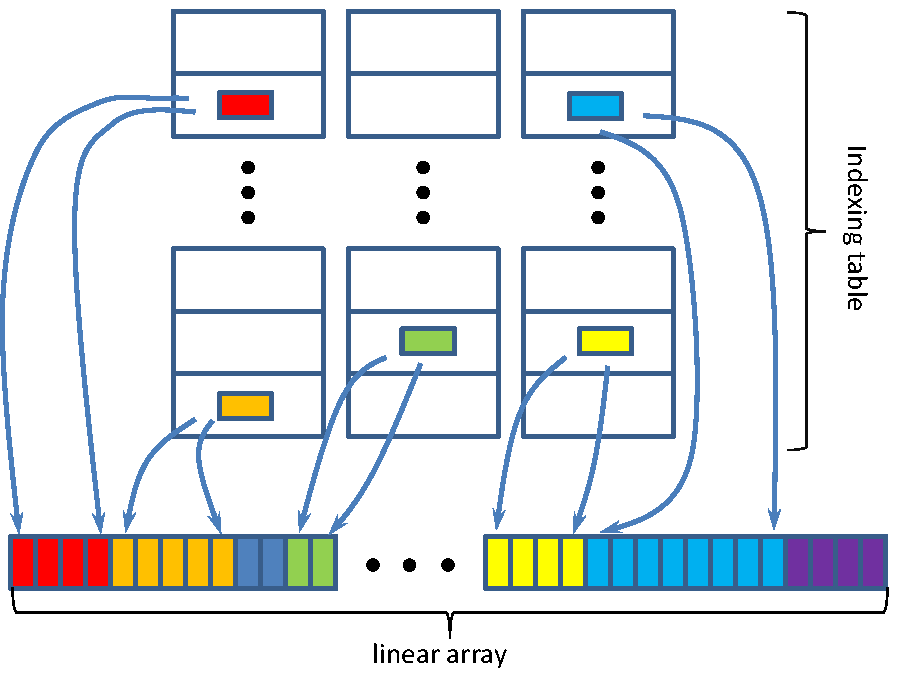
\includegraphics[width=0.8\linewidth]{figs/6/hashtable.pdf}
  \caption[LSH hash table for Bi-level LSH]{\label{fig:6:hashtable} LSH hash table for Bi-level LSH: the linear array stores LSH codes and the indexing table is a cuckoo hash table, which stores unique LSH codes and the intervals for these codes in the linear array. Different colors are for items with different LSH hashing values.}
\end{figure}

Cuckoo hashing~\cite{Pagh:2004:CH} places at most one item at each location in the hash table by allowing items to be moved after their initial placement. It stores the key-value pairs in $f$ hash sub-tables (e.g., $f = 3$ in Figure~\ref{fig:6:hashtable}) with different hash functions for each sub-table. The serial (CPU) implementation inserts items one by one by first checking its $f$ buckets to see any of them is empty. If not, it evicts the old item and replaces it by the new value. The process is repeated recursively until every item finds a position in the table. In theory, a poor choice of hash function could result in a very long time in terms of finding a location for each item, however such cases are rare in practice.
Cuckoo hashing has several advantages over other hashing techniques. First, its space overload is small: the $f$ sub-tables only need $N(1+\gamma)$ memory to store $N$ items with $\gamma = 0.408$. In practice it can achieve about $90\%$ occupancy. Second, cuckoo hashing can provide collision-free storage for $N$ items with very high probability. In practice we can restart cuckoo hashing with different random parameters even after it fails. In practice, the probability that restart is needed is rather low ($0.088\%\sim0.5\%$ for millions of items~\cite{Alcantara:2009:RPH}). Finally, the lookups take only constant time, as only $f$ buckets must be checked. Moreover, the cuckoo hashing is GPU friendly, as it main operations (hashing, insert, evict) are performed in an independent manner for different elements.

In our implementation, we use the GPU cuckoo hashing method proposed in~\cite{Alcantara:2009:RPH}. However, we do not construct a hash table for each data group. Instead, we store all the Bi-level LSH codes in one hash table, because the group index (i.e., the output from RP-tree) can distinguish codes from different groups.

We also enhance the LSH table with a hierarchical structure using Morton curves. The Morton curve maps the multi-dimensional data to a
single dimension and tries to maintain the neighborhood relationship, i.e., nearby points in the high-dimensional space are likely to be close on the one-dimensional curve. Conceptually, the Morton curve can be constructed by recursively
dividing dim-D cube into two cubes and then ordering the cubes, until at most one point resides in each cube. The resulting hierarchical structure is useful in terms of reducing the quality variance among different queries. The Morton curve can be constructed and searched efficiently on the GPU~\cite{LauterbachGSLM09}.


\subsection{Short-list Search}
\label{sec:6:gpu:slsearch}
Short-list search ranks the distances of neighborhood candidates to the query and chooses the $k$ candidates that are closest to the query item. It is usually implemented by inserting the candidates sequentially into a max-heap with the maximum size $k$, which maintains the $k$ best candidates up to this point. Short-list search is the main bottleneck in LSH algorithm and can take more than 95\% of the overall running time.

We describe a GPU-based algorithm to accelerate short-list searches for multiple queries. One naive way is to let each GPU thread handle the short-list search for one query~\cite{Pan:IROS:2010}. This is simple to implement but is not efficient. First, different queries may consider different number of candidates. Such imbalance of tasks will make some threads busy for heap operations, while some other threads are idle and the speed of the overall algorithm is limited by the slowest thread. Second, the max-heap computation is usually implemented on the slow global memory instead of the high-speed shared memory, because the size of max-heap is usually too large for shared memory. Therefore this method can not benefit from shared memory to accelerate data access. Finally, the heap operation (insert, heapify, etc) is related to tree traversal, and is performed in an independent manner for different queries. As a result, instruction divergence and non-coalesced memory accesses will happen among various threads and thereby reduce the overall performance on GPUs.

One possibility is to let each thread perform the heap-insert operation for one candidate for one of the queries. This strategy has been used before to handle multiple collision detection queries on GPUs~\cite{Lauterbach10}. However, in collision detection queries, each thread only traverses one binary tree, but does not update the tree so there are no conflicts among parallel queries. Each thread may add one candidate to the max-heap and may remove another item. Different threads may operate on the same max-heap simultaneously. To avoid any conflicts between multiple threads, we use a heap representation that allows concurrent access of different threads. Most concurrent heap approaches~\cite{Rao:1988:CAP} are based on mutual exclusion, locking part of a heap when inserting or deleting the nodes so that other threads would not access the currently updated element. However, this blocking-based algorithm limits the potential performance to a certain degree, since it involves several drawbacks such as deadlock and starvation, which causes the system to be in idle or wait states. Moreover, it is not easy to implement such lock mechanisms on current CPUs. The lock-free approach~\cite{Sundell:2005:FLC} avoids blocking by using atomic synchronization primitives and guarantees that at least one active operation can be processed. However, lock-free methods~\cite{Sundell:2005:FLC} can be inefficient on current GPUs architectures. Any such algorithm~\cite{Sundell:2005:FLC} needs to synchronize the time that different threads access the heap, which will result in many locks that can involve mutual exclusion and make the operations nearly sequential. Moreover, the algorithm in~\cite{Sundell:2005:FLC} uses the skip-list data structure, which is also difficult to implement efficiently on current GPUs.

Our solution is shown in Figure~\ref{fig:6:workqueue}, which uses work queues allocated on the global memory to accelerate short-list search. Given multiple queries and their candidate sets, we first compute the number of queries that the global memory can handle, i.e., have enough memory for the candidate sets and the initial $k$-nearest neighbors. The initial $k$-nearest neighbors are empty or are the results from previous LSH tables (as introduced in Section~\ref{sec:6:related:basic}, there are $L$ LSH tables). We copy the initial sets and the candidate sets to the work queue and perform clustered-sort on the distances between the points in the work queue and the query points. Finally, we perform a compact operation to obtain updated $k$-nearest neighbor results. This process is repeated until all the candidates have been processed.


\begin{figure}[htb]
  \centering
  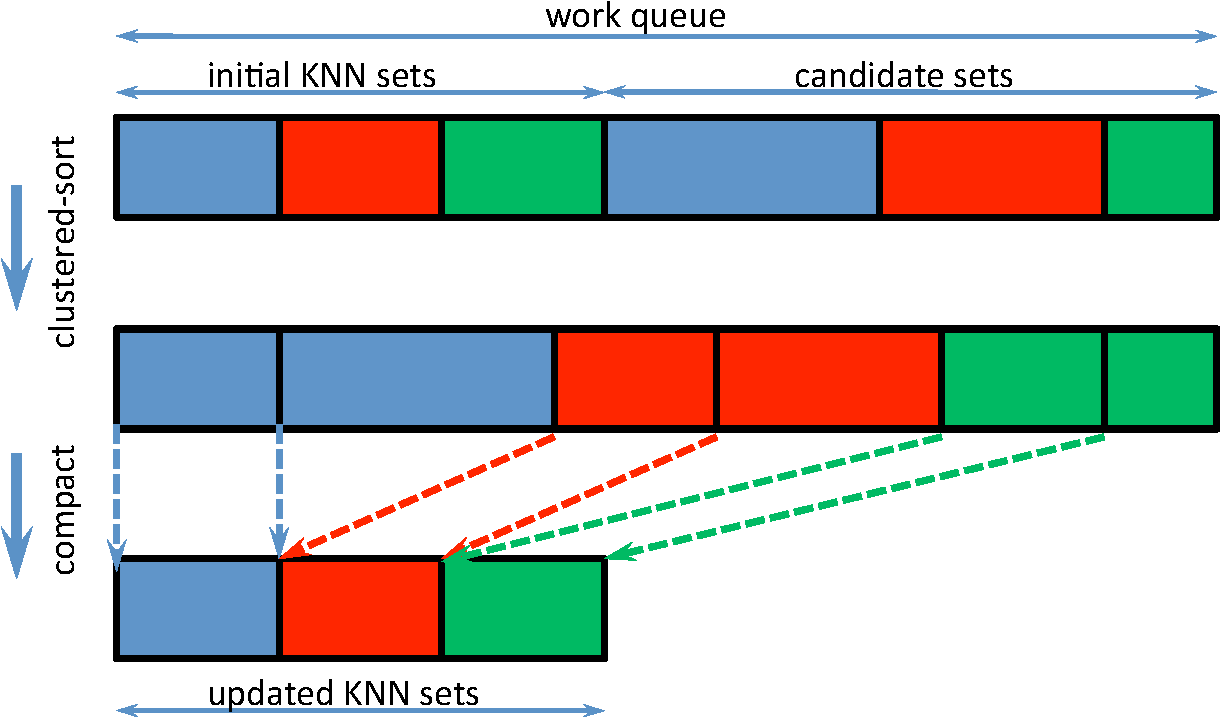
\includegraphics[width=0.8\linewidth]{figs/6/workqueue.pdf}
  \caption[Work queue based parallel short-list search]{\label{fig:6:workqueue} Work queue based parallel short-list search: different colors are for different queries. Clustered-sort collects the candidates for the same query together in the ascending order of distance. Compact primitive computes the first $k$ elements for the reordered candidates, which have the smallest distance to the query. }
\end{figure}

\subsection{Analysis}

Admittedly, sorting on $n$ elements is a more expensive operation than selecting $k$ smallest elements from $n$ elements (which is a special case of the $(n,k)$ multiple-selection problem~\cite{Knuth:1998:ACP}). However, as we show below, our parallel algorithm is \emph{work efficient}~\cite{Joesphbook}, i.e., its complexity is bounded both above and below asymptotically by the complexity of the most efficient serial algorithm for $(n,k)$ multiple-selection.

Suppose we need to solve the $(n,k)$ multiple-selection problem. \cite{Knuth:1998:ACP} gives a complexity lower bound for serial algorithm: $T_S^1(n) \geq n + k + \min(\lfloor (n-k)/2\rfloor, k) -3$
and~\cite{Kaligosi:2005} gives another lower bound: $T_S^2(n) \geq k \ln n + (n-k)\ln\frac{n}{n-k}$.
The complexity of heap-insert based serial algorithm is $T_S^3(n) = \ln k \cdot n$.
Suppose there are $p$ cores available for parallel implementation. According to~\cite{Merrill:2010:RSG}, the complexity of radix sorting on GPU is about $40 n / p$, so our work queue-based parallel method has a complexity $T_P(n) = 40 n / p$.
Obviously, our approach is work efficient and is faster than serial implementations, especially when $k$ is large.

Our approach has many other advantages over the per-thread per-query method. First, it depends on radix sorting, which can benefit the high-speed shared memory and can be implemented efficiently on GPUs.
Second, the timing cost for our method is almost constant when $k$ increases because clustered-sort is performed for all candidates, which is the same for different $k$. The only difference is in the compact step which collects the first $k$ items in the sorted work queue and only takes a small portion of the entire timing cost. The naive heap-sort method's timing cost increases faster than linear when $k$ increases because of the instruction divergence and memory non-coalescence. Moreover, our algorithm behaves much better than the naive method when the number of queries is small. In such cases, the naive method uses only a few threads (the same number as query number) and can not provide enough tasks for GPU cores. Our method performs parallel sorting on the candidates which still utilize all GPU cores. Finally, we can conveniently implement the work queue technique in an out-of-core manner so as to handle very large datasets that cannot fit into the GPU/CPU memory.


\section{Results}
\label{sec:6:res}
In this section, we compare the performance of our Bi-level LSH algorithm with prior LSH methods. All the experiments are performed on a PC with an Intel Core i7 3.2GHz CPU and NVIDIA GTX 480 GPU. The system has 2GB memory and 1GB video memory. The timing results for GPU algorithms already include the time needed to transfer data and results between the CPU and GPU.

To evaluate our method, we use the LabelMe image dataset (\url{http://labelme.csail.mit.edu}), which includes nearly 2 million images and each image is represented as a GIST feature of dimension 512. The Bi-level LSH can provide results with higher quality than prior LSH algorithms, given the same computational budget. We show one comparison result in Figure~\ref{fig:6:res:quality}. More comparison results are shown in~\cite{BilevelLSH2011}.

\begin{figure}[t]
  \centering
  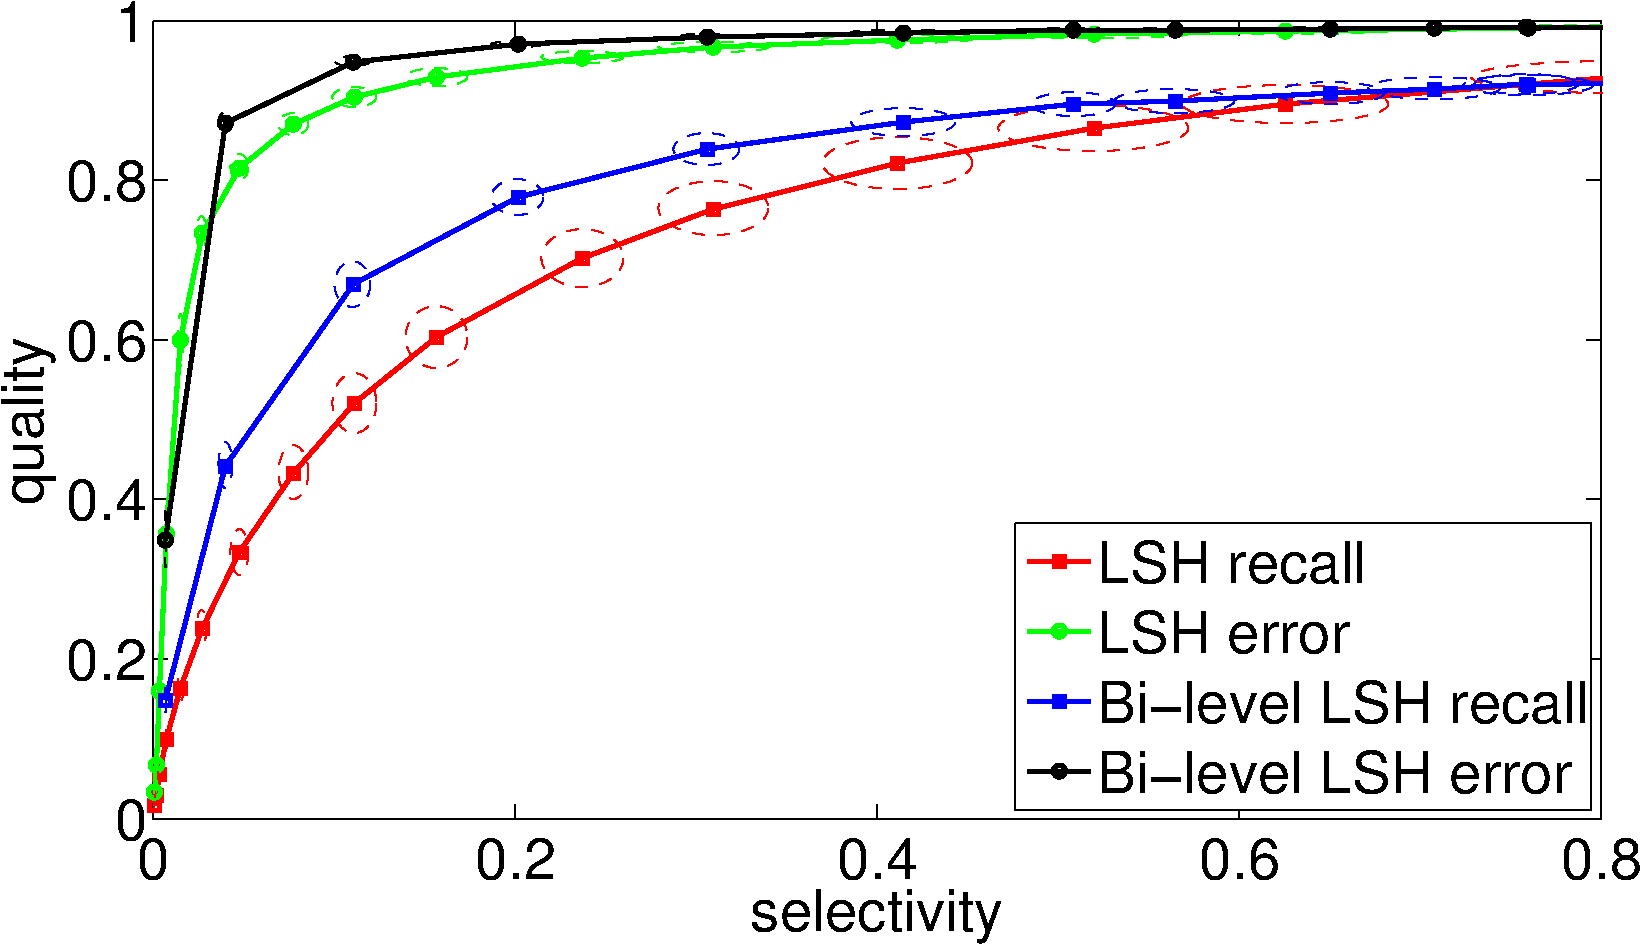
\includegraphics[width=0.8\linewidth]{figs/6/res/compare_L20_mh.pdf}
  \caption[Quality comparison between Bi-level LSH and standard LSH algorithm]{\label{fig:6:res:quality} Quality comparison between our Bi-level LSH and standard LSH algorithm where $M = 8$, and RP-tree partitions the dataset into 16 groups in the first level. The ellipses show the standard variations in selectivity and recall/error ratio caused by random projections.}
\end{figure}

The results on GPU parallelization contains two parts. First, we compare the speed of the naive GPU implementation (i.e., the heap-sort) and the CPU implementations. Next, we show the acceleration over naive GPU implementation obtained using work queues.

For the first level of the Bi-level LSH scheme, the comparison result is shown in Figure~\ref{fig:6:res:level1}. The dataset has 100,000 items and is partitioned into 16 clusters. The K-means algorithm runs for 40 iterations.
For both RP-tree and K-means computations, the GPU implementation is 50-70x faster than a single-core CPU implementation without any SIMD optimizations. We also compare the relative GPU performance for RP-tree and K-means: RP-tree is 2-8 times faster than K-means. The acceleration of RP-tree over K-means will be more for larger datasets.

For the second level of our Bi-level LSH scheme, we compare the efficiency of three approaches. The first is our naive GPU implementation, which uses parallel hash table based on cuckoo hashing to accelerate hash table access and uses parallel heap-sorting for shortlist search. The second approach replaces the parallel shortlist search by serial shortlist search on GPU but still uses parallel hash tables. The final method is based on LSHKIT (\url{http://lshkit.sourceforge.net}), where hash table and shortlist search are implemented on a CPU. In our experiments, we change the bucket size ($W$) to generate different number of shortlist candidates. For different numbers of shortlist candidates, the timing result for the three approaches is shown in Figure~\ref{fig:6:res:shortlist}. The second method is about 2x faster than the third one, where the acceleration is obtained by GPU parallel hash table. The first method is about 15-20x faster than the second one, where the main acceleration is obtained based on GPU shortlist search. Overall, our GPU-based per-thread per-query Bi-Level algorithm can provide 40X acceleration over the CPU implementation.

We now compare the timing performance of two GPU approaches: the naive heap-sort method and the work-queue based method. First, we show their performances when the number of queries changes and the neighborhood size ($K$) is $500$. As shown in Figure~\ref{fig:6:res:workqueuecomp}(a)(b), the work queue based method is about 2-10x faster than the naive heap-sort method when the number of queries is small (i.e., $<$ 10,000) because in such cases naive per-thread per-query strategy cannot provide enough degrees of parallelism so as to benefit from the high number of GPU cores. When the number of queries increase, the speed up of work queue based method over naive method decreases.

Next, we compare the performance of the two approaches when the neighborhood size ($K$) changes. As shown in Figure~\ref{fig:6:res:workqueuecomp}(c)(d), unless $K$ is very small (5 or 50 in the example), work queue-based method is much faster than heap-sort method. When $K$ increases, heap-sort method's timing cost will increase super linearly along with $K$, while work queue-based method almost takes constant time. Figure~\ref{fig:6:res:workqueuecomp}(e) and (f) show the relative comparison between the two approaches, which using a large bucket size ($W$). Notice that work queue-based method is faster than heap-sort method only when $K > 200$ or $K > 500$. The reason is that work queue-based method needs additional memory to store the work queue, which is limited by the overall size of GPU memory. As a result, when $W$ is large, i.e., there are many candidates, we have to split the candidates into many parts so that each part can fit into the work queue. This will break one sorting computation on a work queue into multiple sorting computations, and could reduce the overall efficiency. However, for large $K$, the work queue-based method is still more efficient, which verifies our analysis in Section~\ref{sec:6:gpu:slsearch}.

\begin{figure}[t]
  \subfloat[RP-tree CPU vs. GPU]{
    \centering
    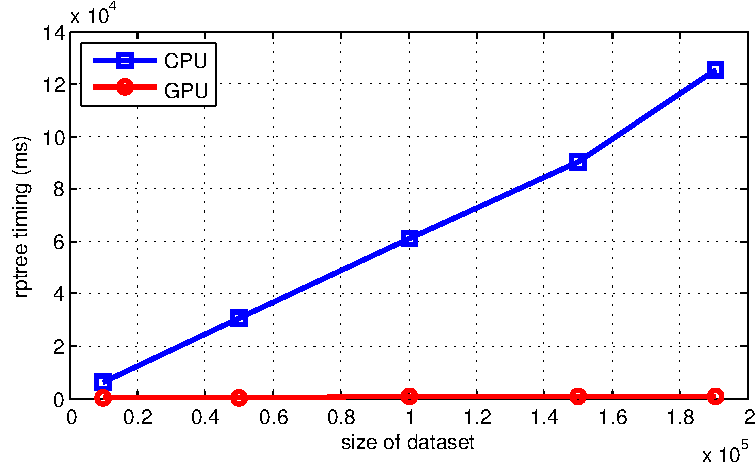
\includegraphics[width=0.327\linewidth]{figs/6/res/rptree_t.pdf}}
  \subfloat[K-means CPU vs. GPU]{
    \centering
    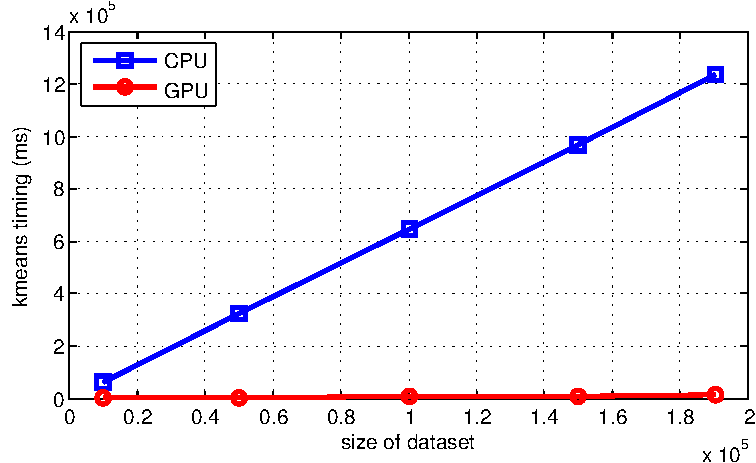
\includegraphics[width=0.327\linewidth]{figs/6/res/kmeans_t.pdf}}
  \subfloat[RP-tree and K-means GPU]{
    \centering
    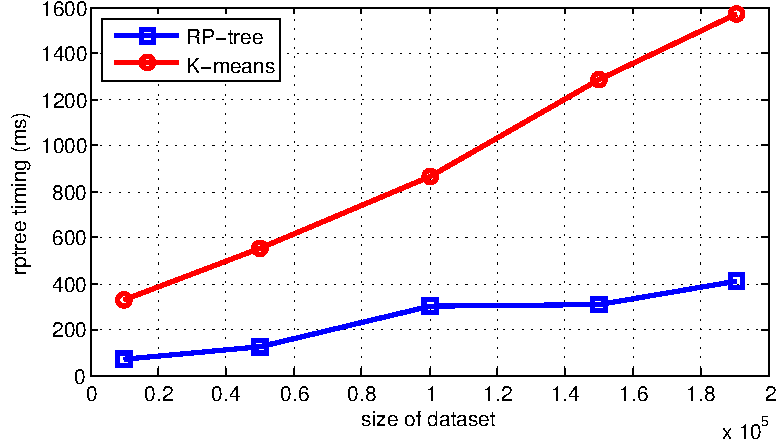
\includegraphics[width=0.327\linewidth]{figs/6/res/rptree_kmeans_gpu.pdf}}
  \caption[Performance comparisons between CPU-based and GPU-based partitioning components in Bi-level LSH]{\label{fig:6:res:level1} Performance comparisons between CPU and GPU on the partitioning algorithm used in Level 1.}
\end{figure}


\begin{figure}[t]
  \centering
  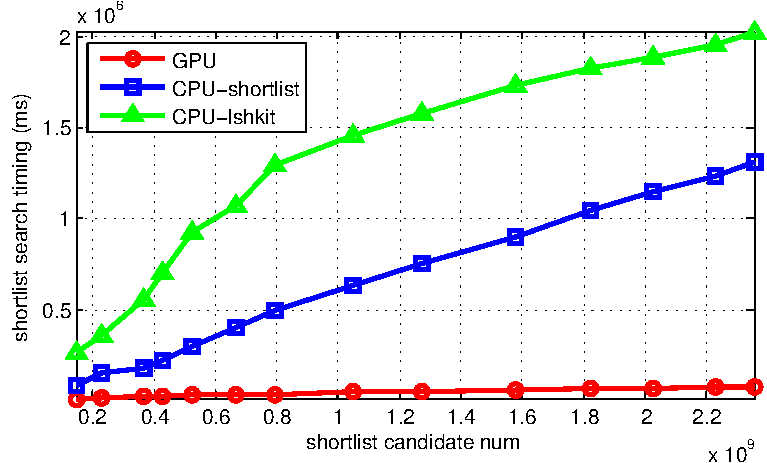
\includegraphics[width=0.8\linewidth]{figs/6/res/shortlist.pdf}
  \caption[Performance comparison on shortlist search used in Bi-level LSH]{\label{fig:6:res:shortlist} Performance comparison on shortlist search: training set size 100,000, testing set size 100,000, set $K=500, L=10, M=8$, change $W$ to generate different number of shortlist candidates. We compare different methods: pure CPU (CPU-lshkit), GPU hash table and CPU short-list search (CPU-shortlist) and pure GPU (GPU).}
\end{figure}


\begin{figure}[t]
  \subfloat[]{
    \centering
    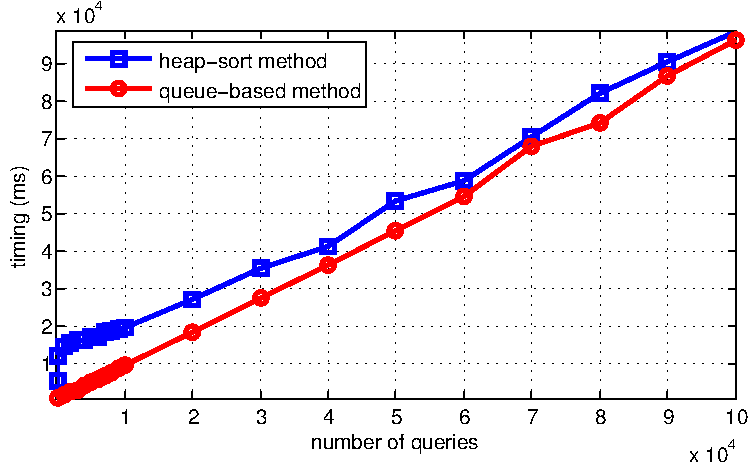
\includegraphics[width=0.327\linewidth]{figs/6/res/workqueue_query.pdf}}
  \subfloat[detail of (a)]{
    \centering
    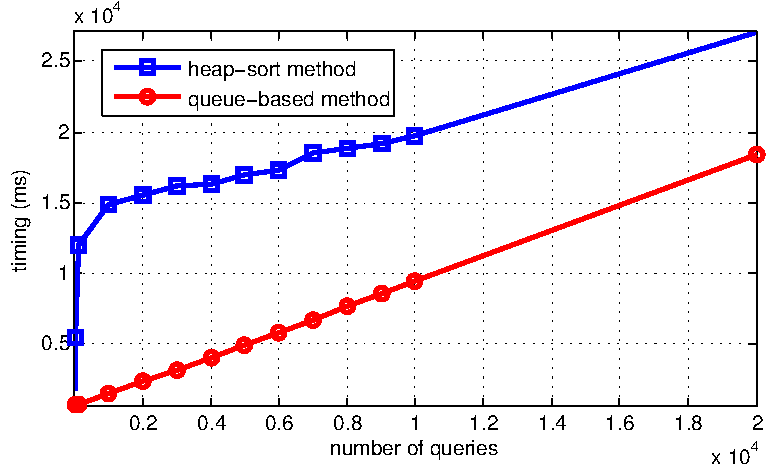
\includegraphics[width=0.327\linewidth]{figs/6/res/workqueue_query_detail.pdf}}
  \subfloat[]{
    \centering
    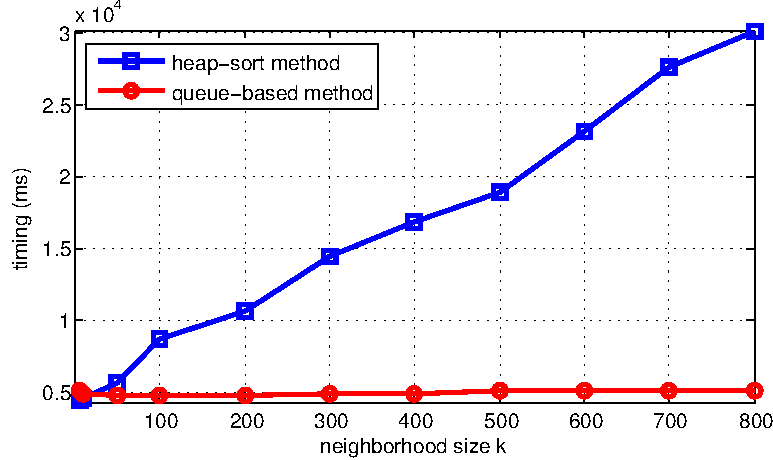
\includegraphics[width=0.327\linewidth]{figs/6/res/workqueue_k_1_W0.pdf}}
    \\
  \subfloat[]{
    \centering
    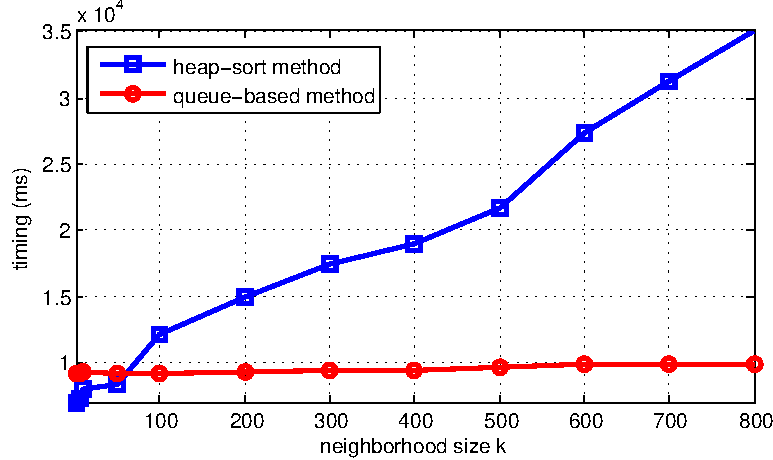
\includegraphics[width=0.327\linewidth]{figs/6/res/workqueue_k_2_W0.pdf}}
  \subfloat[]{
    \centering
    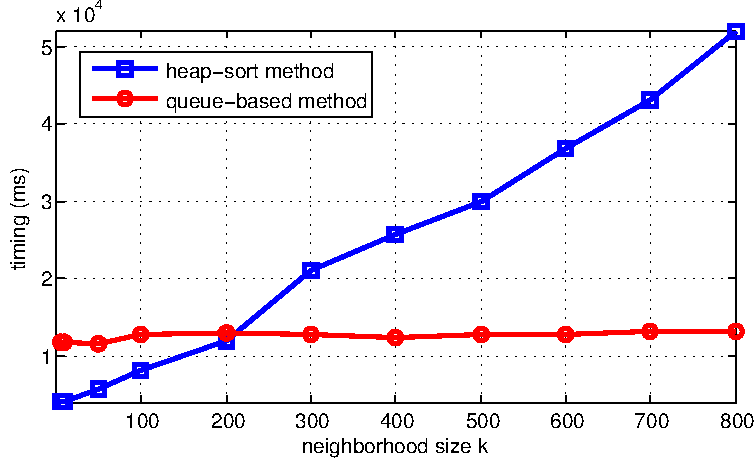
\includegraphics[width=0.327\linewidth]{figs/6/res/workqueue_k_1.pdf}}
  \subfloat[]{
    \centering
    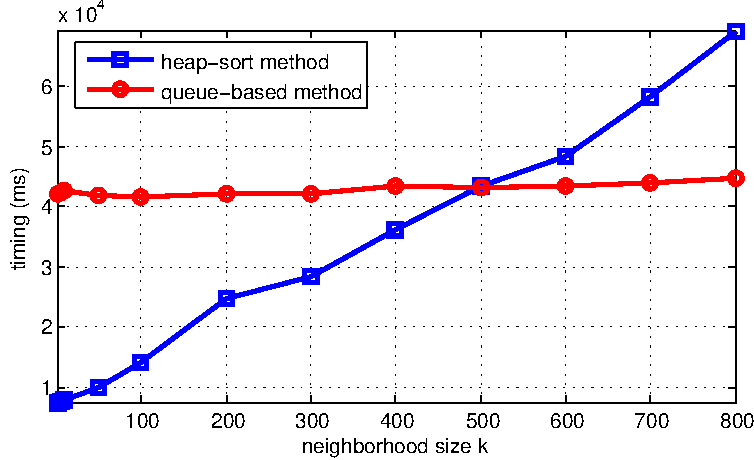
\includegraphics[width=0.327\linewidth]{figs/6/res/workqueue_k_2.pdf}}
\caption[Performance comparison between heap-sort and workqueue-based methods used in Bi-level LSH shortlist search]{\label{fig:6:res:workqueuecomp} Performance comparison on shortlist search between heap-sort and workqueue-based methods: (a) training set size 100,000, test set size changes from 1 to 100,000, $K=500, L=10, M=8, W=W_0$; (b) shows the detail of (a) when change testing set size from 1 to 20,000; (c) training set size 100,000, testing set size 5,000, $L=10, M=8, W=W_0$, $K$ changes from 1 to 800; (d) training set size 100,000, testing set size 10,000, $L=10, M=8, W=W_0$, $K$ changes from 1 to 800; (e) same to (c) except change $W$ to $5W_0$; (f) same to (d) except change $W$ to $5W_0$.}
\end{figure}




\section{Conclusions and Future Work}
We present an efficient GPU-based parallel Bi-level LSH algorithm to perform approximate $k$-nearest neighbor search in high-dimensional space. The Bi-level scheme can provide $k$-nearest neighbor results with higher quality than previous methods. And our parallel algorithm
provides more than 40X acceleration over the LSH algorithms on CPUs.

There are many avenues for future work.  We hope to test our algorithm on more real-world datasets, including images, textures, videos, etc. We also need to design efficient out-of-core algorithms to handle very large datasets (e.g., $>$ 100GB), as the on chip memory on a GPU is limited to few GBs. We need to further analyze the quality of our Bi-Level scheme on large spatial databases.








